\chapter{Introduction}

Unmanned Aerial Vehicles (UAVs) have seen explosive growth in the past thirty years, performing a multitude of military and civilian tasks including surveillance, reconnaissance, armed combat operations, search and rescue, forest fire management, and domestic policing \cite{sarris2001survey, valavanis2007advances}. A class of modern UAVs which have recently grown in popularity are quadrotors -  Vertical Take Off and Landing (VTOL) vehicles powered by four rotors arranged in a cross configuration. The main advantage of the quadrotor lies in its mechanical simplicity. Adjusting the speed of one or more of the vehicle's fixed-pitch rotors provides full attitude control, eliminating the need for the swash plate mechanism found on single rotor helicopters \cite{bramwell2001bramwell, gupte2012survey}. In spite of its mechanical simplicity, the quadrotor exhibits somewhat complex dynamics that are best modeled as a Multi-Input Multi-Output (MIMO) system.

Advances in MEMS sensors and light-weight high-powered lithium polymer batteries have contributed to the recent popularity of quadrotors, making them an attractive choice for research applications in flight dynamics and control, as in \cite{hoffmann2007quadrotor, kivrak2006design, mellinger2010control, michael2010grasp}. One problem of particular interest is the development of mathematical models representing system dynamics based on experimentally gathered data. System identification provides a mechanism to relate this input-output data to the underlying system dynamics. Traditionally, system identification techniques have focused on developing a system model which minimizes prediction error. Identification methods of this form are commonly known as Prediction Error Methods (PEMs). PEMs have seen widespread use in both theoretical and real-world applications, but experience difficulties with MIMO systems as noted in \cite{qin2006overview, viberg1995subspace}. Subspace identification methods have recently grown in popularity and offer an alternative approach to the identification problem. These methods have a foundation in linear algebra and overcome the issues found in PEMs when identifying MIMO systems \cite{katayama2005subspace}. It is the goal of this research project to apply subspace identification techniques to a quadrotor using experimentally gathered closed-loop input and output data.


\section{Related Work}


\begin{figure}[htb!]
	\centering
	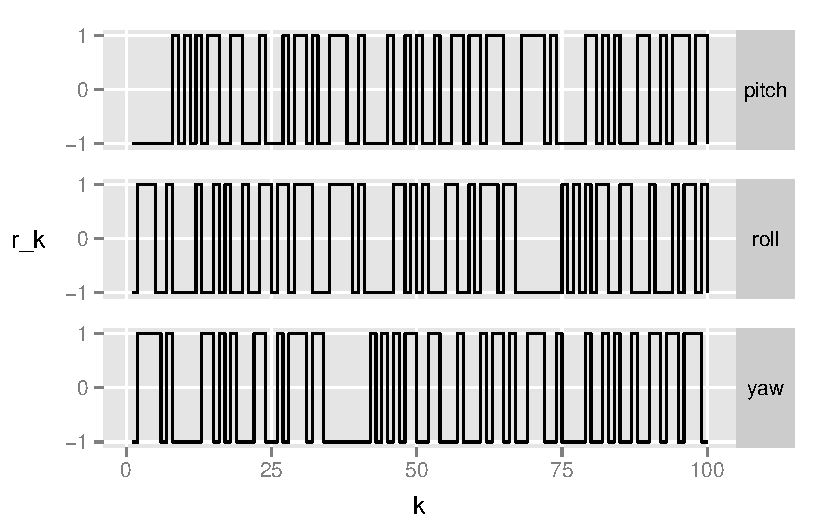
\includegraphics{../fig/prbs_input.pdf}
	\caption{A figure caption}
\end{figure}


\section{Motivation and Contributions}



